% Source: TeX Live PGF manual, pgfmanual-en-tikz-trees.tex, "Missing Children".
\documentclass[border=2pt]{standalone}
\usepackage{tikz}
\usetikzlibrary{trees}

\begin{document}
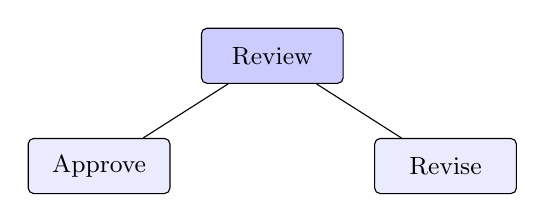
\begin{tikzpicture}[
  grow=down,
  level distance=14mm,
  sibling distance=22mm,
  every node/.style={draw,rounded corners=2pt,minimum width=18mm,minimum height=7mm,fill=blue!8,font=\small}
]
  \node[fill=blue!20] {Review}
    child {node {Approve}}
    child[missing] {node {Escalate}
      child {node {Ignored}}
    }
    child {node {Revise}};
\end{tikzpicture}
\end{document}
